\documentclass[11pt,a4paper]{article}

\usepackage[T1]{fontenc}
\usepackage[utf8]{inputenc}
\usepackage{amsmath,amssymb}
\usepackage{booktabs}
\usepackage{graphicx}
\usepackage{geometry}
\usepackage{hyperref}
\usepackage{parskip}
\usepackage{xcolor}

\geometry{margin=2.5cm}

\hypersetup{
  colorlinks=true,
  linkcolor=blue!60!black,
  urlcolor=blue!60!black,
}

\title{%
  Self-Collision Models for ITER-EDA RF Case 1:\\
  fixed-temperature (\texttt{isc=1}) vs.\ adaptive (\texttt{isc=2})
  Maxwellian background vs.\ the nonlinear operator (\texttt{isc=-1})
}
\author{FP2D\_QLRF\_NL solver --- post-processing analysis}
\date{Version~1.1 \quad\textbullet\quad \today}

\begin{document}

\maketitle
\tableofcontents
\bigskip

\noindent\emph{Revision history.}\;
v1.0 --- initial three-way comparison, $D_{\perp\perp}/F_\perp$ diagnostics and
mechanism.\;
v1.1 --- adds the carried-out diagnostic tests (Section~\ref{sec:tests}:
common-$f$ operator comparison, velocity-space SC power density, and the
$P_\text{SC}$ time traces with the self-collision timescale), and refines the
discussion of the fixed-temperature model.
\bigskip

% ---------------------------------------------------------------------------
\section{Case Setup}
% ---------------------------------------------------------------------------

This is a \emph{pure ICRF} case: there is no particle source
(\texttt{isource=0}). The simulation evolves a tritium minority ($A=3$, $Z=1$)
that starts from a Maxwellian at $T = 12$\,keV (thermal equilibrium with the
bulk) and is heated at the 2nd cyclotron harmonic (60.9\,MHz; $f_c=30.5$\,MHz).
The background is a deuterium plasma at $T = 12$\,keV and
$n_e = 1.5\times10^{20}$\,m$^{-3}$; the tritium fraction is $x_T = 0.5$
($n_T = 7.5\times10^{19}$\,m$^{-3}$). The velocity-space
grid is $150\times150$ in $(v_\perp, v_\parallel)$, with
$v_\perp^{\max} = 3.5\times10^{7}$\,m\,s$^{-1}$ and
$v_\parallel^{\max} = 4\times10^{6}$\,m\,s$^{-1}$.

\textbf{The three runs use identical solver parameters} --- same grid, same
two-phase time stepping (\texttt{ntimes}\,=\,600,\,2000;
\texttt{timestep}\,=\,1\,ms,\,25\,ms), same initial condition
(\texttt{iold=0}, \texttt{istart=1}, i.e.\ the $T=12$\,keV Maxwellian), and
same convergence tolerance ($10^{-4}$). They differ \emph{only} in the
self-collision flag \texttt{isc}. Any difference in the results is therefore
attributable solely to the self-collision model, not to the numerical
settings.

% ---------------------------------------------------------------------------
\section{Self-Collision Models}
% ---------------------------------------------------------------------------

\subsection{Nonlinear operator (\texttt{isc=-1})}

The fully nonlinear operator uses the actual distribution $f$ as both the
test-particle and the field (background) distribution:
\begin{equation}
  C[f,f] = \nabla_v \cdot
    \left[ \mathbf{A}(f)\,f - \mathbf{D}(f)\cdot\nabla_v f \right],
\end{equation}
where the friction vector $\mathbf{A}$ and diffusion tensor $\mathbf{D}$ are
functionals of $f$ through the Rosenbluth potentials. This operator satisfies
\emph{exact energy conservation}:
\begin{equation}
  \int C[f,f]\;\tfrac{1}{2}m v^2\; d^3v \equiv 0 \qquad \forall\, f.
\end{equation}

\subsection{Linearised operators (\texttt{isc=1} and \texttt{isc=2})}

Both Maxwellian-background models replace the field distribution by an
isotropic Maxwellian $f_M(T_b)$ and use the \emph{same} linearised operator
$C[f, f_M(T_b)]$, computed analytically (Chandrasekhar function) in
\texttt{cblin}. They differ \emph{only} in the choice of the background
temperature $T_b$:
\begin{align}
  \texttt{isc=1}:&\quad T_b = T_\text{Stix} = 12~\text{keV (fixed, the bulk
    temperature)},\\
  \texttt{isc=2}:&\quad T_b = T_\text{eff}(t) = \frac{2T_\perp + T_\parallel}{3}
    \quad\text{(evolving with the minority's own energy)}.
\end{align}
The Maxwellian background is
\begin{equation}
  f_M(v; T_b) = \frac{n}{\pi^{3/2} v_\text{th}^3}
    \exp\!\left(-\frac{v^2}{v_\text{th}^2}\right),
  \qquad
  v_\text{th} = 9.79\times10^3\sqrt{T_b[\text{eV}]/A}.
\end{equation}

A key point for what follows: \emph{neither} linearised operator conserves
energy exactly when $f \neq f_M(T_b)$, because the background acts as an
external reservoir of infinite heat capacity. The energy moment
\begin{equation}
  P_\text{SC} = \int C[f, f_M(T_b)]\;\tfrac{1}{2}mv^2\;d^3v
  \label{eq:psc}
\end{equation}
is the net collisional energy transfer between $f$ and that reservoir. Its
sign and magnitude depend critically on $T_b$, as the results below show.

% ---------------------------------------------------------------------------
\section{Results}
% ---------------------------------------------------------------------------

\subsection{Final-state summary}

\begin{table}[h]
\centering
\caption{Final-state diagnostics for the three runs (identical solver
  settings). Powers in MW\,m$^{-3}$.}
\label{tab:results}
\begin{tabular}{lccc}
\toprule
Quantity & \texttt{isc=1} (NLMax1) & \texttt{isc=2} (NLMax2) & \texttt{isc=-1} (NLSC) \\
         & fixed $T_b=12$\,keV     & adaptive $T_b=T_\text{eff}$ & exact \\
\midrule
Converged?                  & Yes (step 945)  & Yes (step 1374) & No (plateau)\footnotemark \\
$T_\text{eff}$ (keV)        & \textbf{19.4}   & \textbf{78.9}   & \textbf{22.2} \\
$\langle E_\text{kin}\rangle$ (keV) & 29.1    & 118.3           & 33.3 \\
$E_\perp$ (keV)             & 22.8            & 105.3           & 26.6 \\
$E_\parallel$ (keV)         & 6.34            & 13.0            & 6.71 \\
Anisotropy                  & 64.2\%          & 80.1\%          & 66.5\% \\
\midrule
$P_\text{RF}$               & 1.128           & 3.413           & 1.247 \\
$P_\text{coll,e}$           & $-0.271$        & $-2.430$        & $-0.372$ \\
$P_\text{coll,D}$           & $-0.477$        & $-4.486$        & $-0.872$ \\
$P_{\mathrm{SC},\perp}$     & $-0.394$        & $+2.131$        & $-0.137$ \\
$P_{\mathrm{SC},\parallel}$ & $+0.014$        & $+1.359$        & $+0.135$ \\
$P_{\mathrm{SC,total}}$     & $\mathbf{-0.380}$ & $\mathbf{+3.490}$ & $\mathbf{-0.002}$ \\
Power balance residual      & $-2.2\times10^{-4}$ & $-1.3\times10^{-2}$ & $-1.6\times10^{-4}$ \\
\bottomrule
\end{tabular}
\end{table}
\footnotetext{The \texttt{isc=-1} run does not formally converge: $dE/E$
  plateaus at $\approx 4.2\times10^{-4}$, just above the $10^{-4}$ tolerance,
  while the power residual $dP/P_d \sim 10^{-7}$ is fully converged. This is a
  numerical floor of the energy-norm estimator for the nonlinear operator, not
  ongoing physical evolution: $T_\text{eff}$ is stationary to within
  $0.1$\,keV over the last 1000 steps.}

\subsection{The central observation}

\texttt{isc=1} tracks the exact operator (\texttt{isc=-1}) closely \emph{at
steady state}: $T_\text{eff} = 19.4$ vs.\ $22.2$\,keV,
$P_\text{RF} = 1.13$ vs.\ $1.25$\,MW\,m$^{-3}$, anisotropy $64$ vs.\ $67$\%.
\texttt{isc=2}, by contrast, is wildly off: $T_\text{eff} = 79$\,keV (a factor
$\sim$3.5 too hot) and $P_\text{RF}$ a factor $\sim$3 too large. (As Test~1 in
Section~\ref{sec:tests} shows, this steady-state agreement does \emph{not} mean
the \texttt{isc=1} operator is locally accurate --- only that its error has a
benign sign.)

This is the result that demands explanation, because \texttt{isc=1} and
\texttt{isc=2} use the \emph{same} linearised operator and differ only in
$T_b$. The failure of \texttt{isc=2} therefore \emph{cannot} be attributed to
the linearisation itself, nor to the fact that $f$ is non-Maxwellian (both
models see the same non-Maxwellian $f$). The culprit must be the choice
$T_b = T_\text{eff}$.

The time evolution of $T_\text{eff}$ (Fig.~\ref{fig:teff}) makes the contrast
vivid. \texttt{isc=1} and \texttt{isc=-1} both rise from $12$\,keV and level
off near $19$--$22$\,keV within $\sim$2\,s, whereas \texttt{isc=2} climbs
monotonically through these values without arrest, passing $77$\,keV and still
rising at the right edge of the plot.

\begin{figure}[h]
  \centering
  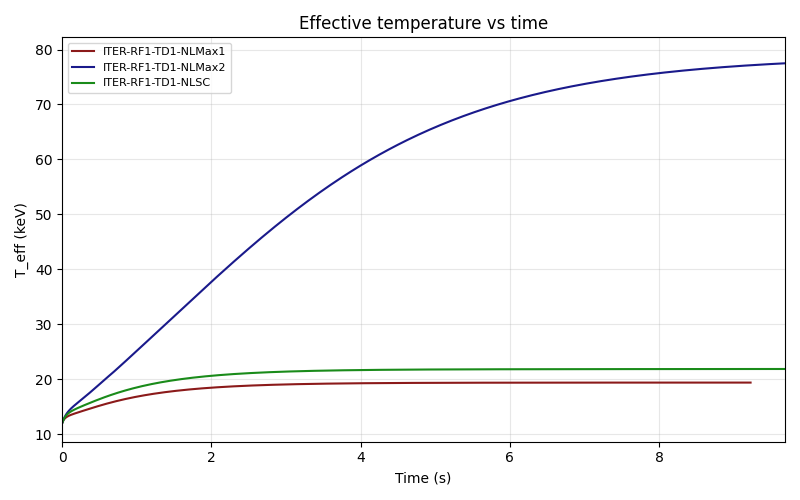
\includegraphics[width=0.78\textwidth]{comp_teff.png}
  \caption{Effective temperature $T_\text{eff}(t)$ for the three runs.
    \texttt{isc=1} (NLMax1, red) and \texttt{isc=-1} (NLSC, green) saturate
    close together at $\approx 19$ and $22$\,keV; \texttt{isc=2} (NLMax2,
    blue) runs away monotonically, reaching $\approx 79$\,keV at its own
    (later) convergence. The horizontal axis is truncated at the \texttt{isc=1}
    convergence time ($t \approx 9.2$\,s), where the \texttt{isc=2} curve is
    still climbing.}
  \label{fig:teff}
\end{figure}

\subsection{Self-collision power: the sign tells the story}

The energy moment $P_\text{SC}$, Eq.~\eqref{eq:psc}, behaves qualitatively
differently in the three cases:
\begin{description}
  \item[\texttt{isc=-1}: $P_\text{SC} \approx -0.002$\,MW\,m$^{-3}$ ($\approx 0$).]
    Energy-conserving to numerical precision. The split
    $P_{\mathrm{SC},\perp} = -0.137$,
    $P_{\mathrm{SC},\parallel} = +0.135$ shows pure redistribution
    (pitch-angle scattering / isotropisation) with no net energy change.
  \item[\texttt{isc=1}: $P_\text{SC} = -0.380$\,MW\,m$^{-3}$ (sink).]
    A modest \emph{negative} (cooling) term. The cold $12$\,keV background
    drags the RF-heated minority back toward the bulk. This opposes the RF
    drive --- it is \emph{stabilising} --- and the steady state settles close
    to the true one.
  \item[\texttt{isc=2}: $P_\text{SC} = +3.490$\,MW\,m$^{-3}$ (source).]
    A large \emph{positive} (heating) term, comparable to the entire RF
    input. The self-collision operator behaves as an energy source. This is
    \emph{destabilising} and drives the runaway.
\end{description}

% ---------------------------------------------------------------------------
\section{Diffusion and friction diagnostics}
% ---------------------------------------------------------------------------

To pinpoint the mechanism we output, at the end of each run, the
perpendicular diffusion coefficient $D_{\perp\perp}$ and the perpendicular
friction $F_\perp$ of the self-collision operator along the $v_\parallel = 0$
slice. For \texttt{isc=1,2} these come directly from \texttt{cblin}
($D_{\perp\perp} = \Theta + v_\parallel^2\Phi$, $F_\perp = -v_\perp\Psi$); for
\texttt{isc=-1} they are reconstructed from the numerically-computed
Rosenbluth potentials ($D_{\perp\perp} = -\tfrac{4\pi\gamma}{n}\,
\partial^2\psi/\partial v_\perp^2$,
$F_\perp = -\tfrac{4\pi\gamma}{n}\,\partial\phi/\partial v_\perp$).

\begin{figure}[h]
  \centering
  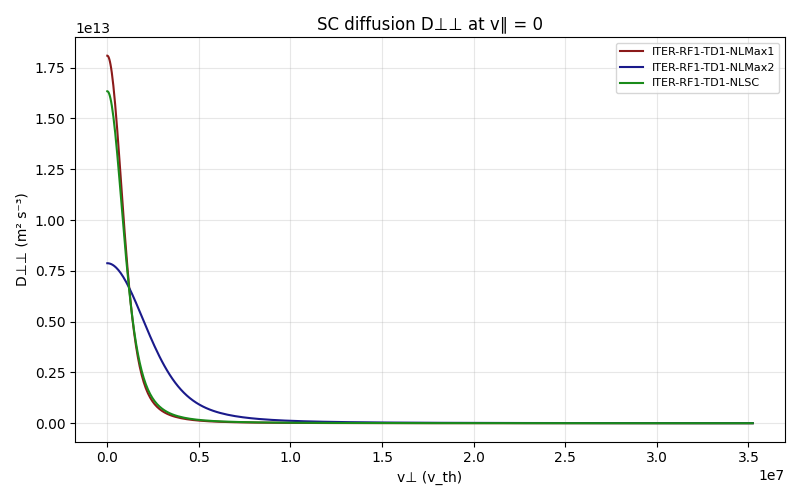
\includegraphics[width=0.49\textwidth]{../Dpepe_comp.png}\hfill
  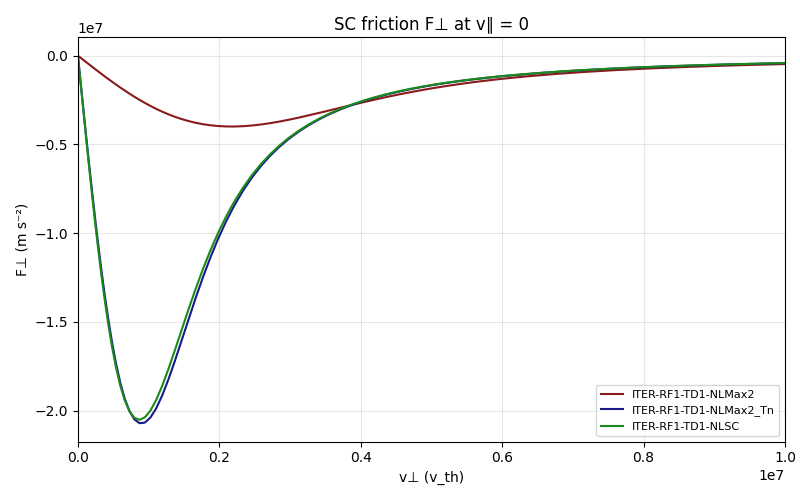
\includegraphics[width=0.49\textwidth]{../Fpe_comp.png}
  \caption{Self-collision perpendicular diffusion $D_{\perp\perp}$ (left) and
    friction $F_\perp$ (right) at $v_\parallel = 0$, for the final state of
    each run. \texttt{isc=1} (red) and \texttt{isc=-1} (green) nearly
    coincide; \texttt{isc=2} (blue) is qualitatively different: its diffusion
    is lower at the axis but far broader in $v_\perp$, and its friction is
    $\sim$5$\times$ weaker with its minimum displaced to higher $v_\perp$.}
  \label{fig:dpepe_fpe}
\end{figure}

The diagnostics (Fig.~\ref{fig:dpepe_fpe}) are unambiguous:

\begin{itemize}
  \item \textbf{\texttt{isc=1} and \texttt{isc=-1} coincide.} Both
        $D_{\perp\perp}$ (peak $\approx 1.7$--$1.8\times10^{13}$\,m$^2$\,s$^{-3}$
        at the axis, decaying to zero by $v_\perp \approx 5$\,Mm\,s$^{-1}$) and
        $F_\perp$ (deep well, minimum $\approx -2\times10^{7}$\,m\,s$^{-2}$ at
        $v_\perp \approx 0.8$\,Mm\,s$^{-1}$) are essentially the same for the
        fixed-$12$\,keV background and the exact operator.

  \item \textbf{\texttt{isc=2} is qualitatively wrong.} Its diffusion peak is
        less than half ($\approx 0.8\times10^{13}$) but \emph{extends far out
        in $v_\perp$} --- significant diffusion persists out to
        $v_\perp \approx 10$\,Mm\,s$^{-1}$, where the other two have vanished.
        Its friction well is $\sim$5$\times$ shallower
        ($\approx -0.4\times10^{7}$) and displaced outward to
        $v_\perp \approx 2$\,Mm\,s$^{-1}$.
\end{itemize}

% ---------------------------------------------------------------------------
\section{Physical Interpretation}
% ---------------------------------------------------------------------------

\subsection{Density-weighted field vs.\ energy-weighted temperature}

The friction and diffusion felt by a test particle are
\emph{number-density-weighted} integrals over the field particles (the
Rosenbluth potentials are convolutions of $f$ with $|v-v'|$ and $1/|v-v'|$).
They are therefore dominated by the \emph{dense, cold bulk} of the
distribution, not by the sparse high-energy tail. The bulk of the minority,
even after RF heating, remains close to the $12$\,keV core, because the RF
populates a thin perpendicular tail that carries much energy but little
particle number.

This is precisely why \texttt{isc=1} works (Fig.~\ref{fig:dpepe_fpe}): a fixed
Maxwellian at the \emph{bulk} temperature ($12$\,keV) is an excellent proxy
for the true collisional field, because the true field is set by the bulk. The
fixed-background operator is, in effect, an extra drag against a cold thermal
population --- physically equivalent to an additional bulk-ion collision
channel, with the stabilising (cooling) sign. This agreement concerns the
$D_{\perp\perp}/F_\perp$ \emph{shapes} near the bulk and the self-consistent
steady state; applied to a \emph{fixed} $f$ the energy moment of the
\texttt{isc=1} operator still differs markedly from the exact one (it is a
sizeable sink, not $\approx0$) --- see Test~1, Section~\ref{sec:tests}.

$T_\text{eff} = (2T_\perp + T_\parallel)/3$, on the other hand, is an
\emph{energy-weighted} moment. It is pulled up to $79$\,keV by the
perpendicular RF tail. Using $T_\text{eff}$ as the background temperature
(\texttt{isc=2}) therefore characterises the collisional field by the hot
tail rather than the cold bulk --- the wrong weighting entirely. The
background Maxwellian is made $\sim$6$\times$ too hot, so
$v_\text{th}(T_b)$ is $\sim$2.5$\times$ too large, which directly produces the
broad diffusion and weak friction seen in Fig.~\ref{fig:dpepe_fpe}.

\subsection{Why \texttt{isc=2} becomes an energy source}

The equilibrium of a linearised operator is $f = f_M(T_b)$, enforced by the
fluctuation--dissipation balance between friction and diffusion,
$F_\perp / D_{\perp\perp} \sim v_\perp / v_\text{th}^2(T_b)$. Lowering this
ratio (hotter background) means the operator relaxes $f$ toward a hotter
target. Concretely, in \texttt{isc=2}:
\begin{itemize}
  \item the broad $D_{\perp\perp}$ keeps up-scattering particles in the
        perpendicular tail (injecting $\perp$ energy) far out in $v_\perp$,
        where it should have died away;
  \item the friction $F_\perp$, suppressed $\sim$5$\times$, is far too weak to
        pull those particles back.
\end{itemize}
The net perpendicular energy moment is therefore strongly positive
($P_{\mathrm{SC},\perp} = +2.13$\,MW\,m$^{-3}$), and the operator acts as a
heating source rather than a relaxation term. Because $T_b = T_\text{eff}$ is
slaved to the minority's own energy, this closes a positive feedback loop:
\begin{equation*}
  T_\text{eff}\uparrow
  \;\longrightarrow\; T_b = T_\text{eff}\uparrow
  \;\longrightarrow\; F_\perp/D_{\perp\perp}\downarrow
  \;\longrightarrow\; P_\text{SC}\uparrow
  \;\longrightarrow\; T_\text{eff}\uparrow\uparrow.
\end{equation*}
There is no restoring force. $T_\text{eff}$ runs up until the genuine Coulomb
losses to electrons and bulk D ions --- which scale with $T_\text{eff}$ and do
\emph{not} share this feedback --- grow large enough to balance the spurious
source, which happens only at $T_\text{eff} \approx 79$\,keV.

In \texttt{isc=1} the same fluctuation--dissipation argument runs the other
way: the fixed cold background gives strong friction and narrow diffusion, so
the operator relaxes $f$ toward the $12$\,keV bulk, removing energy
($P_\text{SC} < 0$). This is a stable negative feedback and the steady state
stays close to the true one.

\subsection{Why \texorpdfstring{$P_\text{RF}$}{P\_RF} tracks \texorpdfstring{$T_\text{eff}$}{Teff}}

The inflated $P_\text{RF}$ in \texttt{isc=2} is a \emph{secondary}
consequence, not an independent effect. The 2nd-harmonic quasilinear
absorption scales with the number of resonant ions and the Bessel overlap
$J_1^2(k_\perp v_\perp/\Omega_c)$. The artificially hot, broad perpendicular
distribution places far more ions in resonance, so $P_\text{RF}$ grows with
$T_\text{eff}$ and feeds the same runaway. The factor-3 excess in
$P_\text{RF}$ is thus downstream of the factor-3.5 excess in $T_\text{eff}$.

% ---------------------------------------------------------------------------
\section{Diagnostic tests}
\label{sec:tests}
% ---------------------------------------------------------------------------

Three of the diagnostics suggested in the previous version have been carried
out. They confirm the mechanism and sharpen one point about the
fixed-temperature model.

\subsection{Test 1 --- the three operators on a common \texorpdfstring{$f$}{f}}

Evaluating all three self-collision operators on the \emph{same} distribution
(the converged \texttt{isc=-1} VDF, $T_\text{eff}\approx22$\,keV) removes the
confound of the different final states (Table~\ref{tab:commonf}).

\begin{table}[h]
\centering
\caption{Self-collision power (MW\,m$^{-3}$) of each operator applied to the
  single common distribution $f$ (the converged \texttt{isc=-1} VDF).}
\label{tab:commonf}
\begin{tabular}{lccc}
\toprule
Operator on common $f$ & $P_{\mathrm{SC},\perp}$ & $P_{\mathrm{SC},\parallel}$ & $P_{\mathrm{SC,total}}$ \\
\midrule
\texttt{isc=-1} (exact)                      & $-0.138$ & $+0.136$ & $\approx 0$ \\
\texttt{isc=1} ($T_b=12$\,keV)               & $-0.624$ & $-0.077$ & $-0.70$ \\
\texttt{isc=2} ($T_b=T_\text{eff}=22$\,keV)  & $+1.70$  & $+1.38$  & $+3.08$ \\
\bottomrule
\end{tabular}
\end{table}

The exact operator conserves energy ($\approx0$) and merely transfers
$\perp\!\to\!\parallel$ (isotropisation of the RF-driven anisotropy). Both
linearised operators, applied to this \emph{same} $f$, are far off:
\texttt{isc=1} is a large \emph{sink} ($-0.70$) and \texttt{isc=2} a large
\emph{source} ($+3.08$).

This is the key refinement of v1.1. The good steady-state agreement of
\texttt{isc=1} (Table~\ref{tab:results}) is \emph{not} because the
fixed-temperature operator is locally accurate --- on a fixed $f$ it is not.
It is because its error has the \emph{stabilising} sign (a drag/sink): the run
self-adjusts to a slightly cool but stable equilibrium where RF input balances
the over-strong collisional loss. \texttt{isc=2}'s error has the opposite,
\emph{destabilising} sign (a source), for which no stable balance exists ---
hence the runaway. The opposite signs follow directly from the background
temperature relative to the distribution: $f$ has $T_\text{eff}=22$\,keV
(energy-weighted, inflated by the perpendicular tail) but a particle bulk still
near $12$\,keV, so the $12$\,keV bath of \texttt{isc=1} cools the tail while the
$22$\,keV bath of \texttt{isc=2} heats the bulk.

\subsection{Test 2 --- velocity-space density of the SC power}

Figure~\ref{fig:scpd_maps} maps
$dP_\text{SC}/d^3v = \tfrac12 m v^2\,C_\text{SC}[f]$ (source $>0$, sink $<0$)
for each run; Fig.~\ref{fig:scpd_slice} compares the $v_\parallel=0$ slices.

\begin{figure}[h]
  \centering
  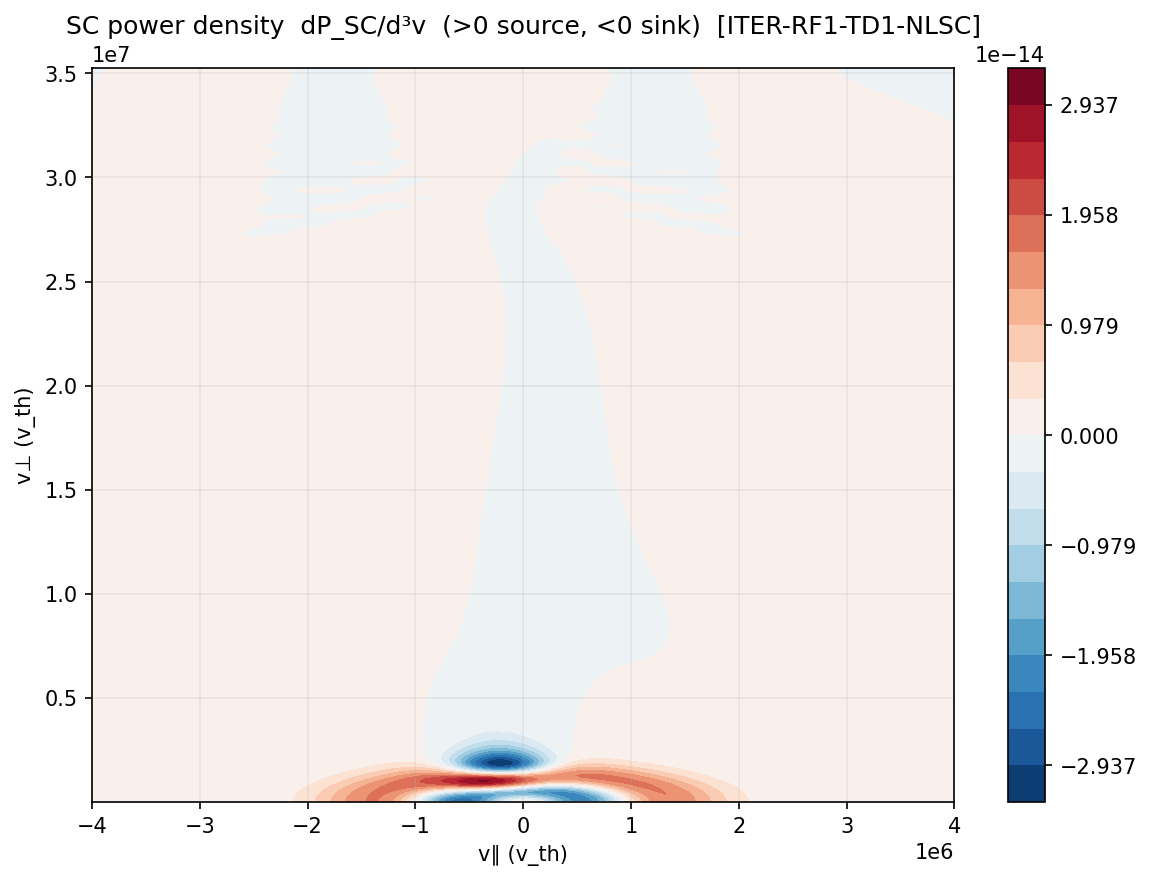
\includegraphics[width=0.32\textwidth]{../sc_power_density-ITER-RF1-TD1-NLSC.png}\hfill
  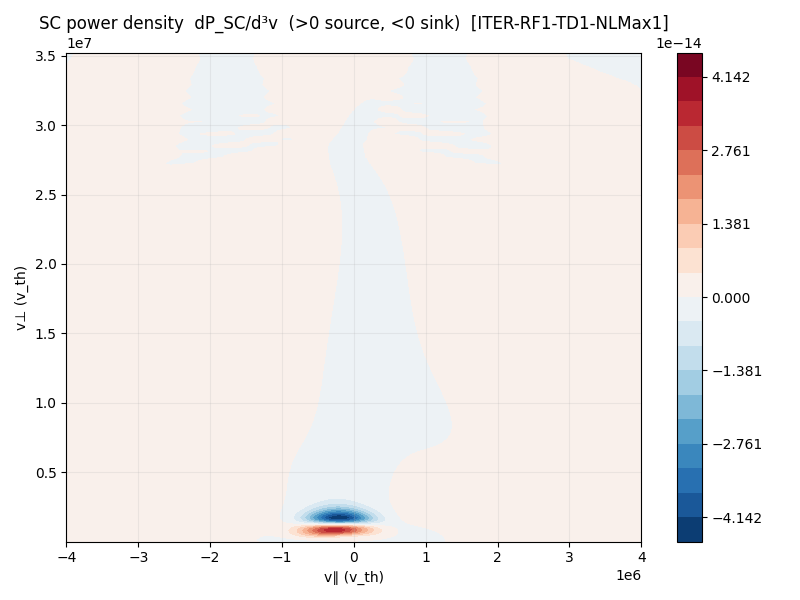
\includegraphics[width=0.32\textwidth]{../SC_power_density-NLMax1.png}\hfill
  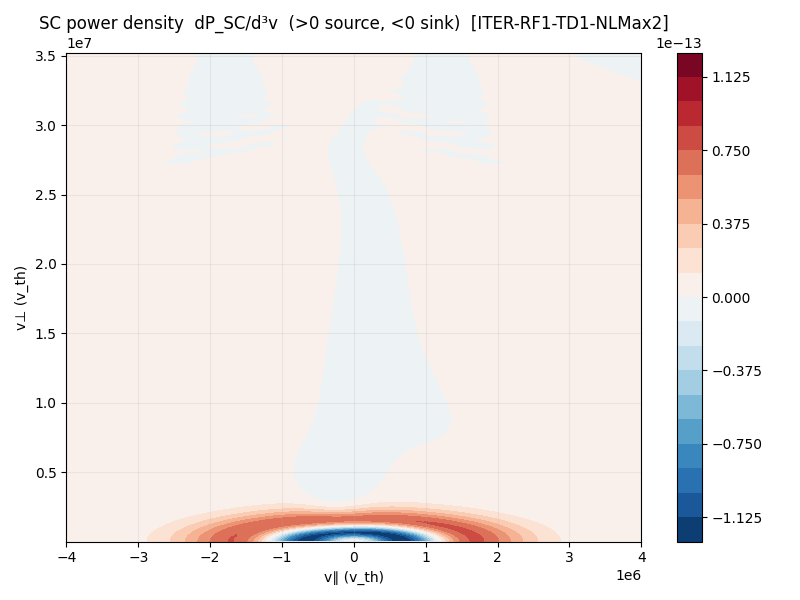
\includegraphics[width=0.32\textwidth]{../SC_power_density-NLMax2.png}
  \caption{SC power density $dP_\text{SC}/d^3v$ for \texttt{isc=-1} (left),
    \texttt{isc=1} (centre) and \texttt{isc=2} (right). \texttt{isc=-1} and
    \texttt{isc=1} are tightly localised at the bulk (a dipolar pitch-angle
    pattern; net $\approx0$ and net sink respectively). \texttt{isc=2} shows a
    broad \emph{source} band spread in $v_\parallel$ and reaching up in
    $v_\perp$, with a sink core at $v_\parallel\approx0$.}
  \label{fig:scpd_maps}
\end{figure}

\begin{figure}[h]
  \centering
  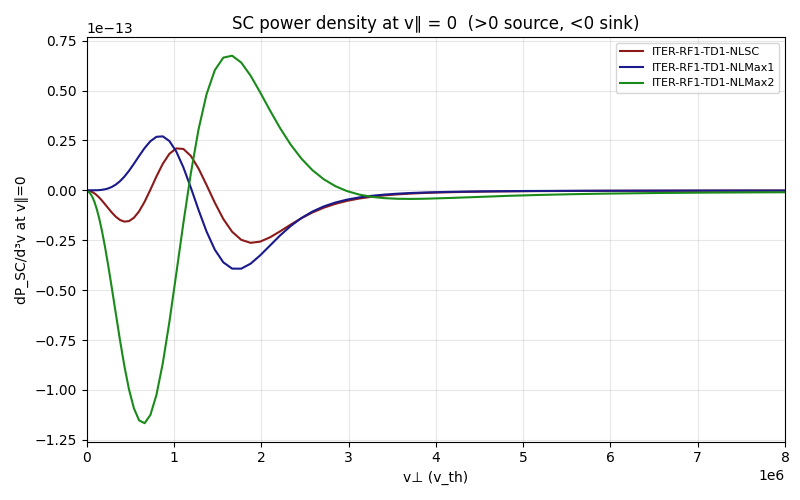
\includegraphics[width=0.70\textwidth]{../SC_power_density_at_vpar0-comps_zoom.png}
  \caption{$dP_\text{SC}/d^3v$ at $v_\parallel=0$. \texttt{isc=2} (green) has a
    large positive lobe at $v_\perp\approx1.6$\,Mm\,s$^{-1}$ --- a perpendicular
    \emph{source} in the bulk --- absent in \texttt{isc=-1} (red) and
    \texttt{isc=1} (blue).}
  \label{fig:scpd_slice}
\end{figure}

\paragraph{Why \texttt{isc=2} becomes a \emph{perpendicular} source.}
A collisional operator drives the local logarithmic slope of $f$ toward that
of its background Maxwellian (the fluctuation--dissipation balance
$D\,\partial_v f + F f \to 0$, i.e.\
$\partial_v\ln f \to -2v/v_\text{th}^2(T_b)$). Where $f$ is \emph{colder} than
$T_b$ (steeper than $f_M(T_b)$) diffusion beats friction and particles are
scattered \emph{up} in energy (source); where $f$ is hotter than $T_b$,
friction wins (sink). For \texttt{isc=2}, $T_b=T_\text{eff}=22$\,keV sits
\emph{above} the bulk core ($\sim$12\,keV), so across the densely populated
bulk $f$ is colder than the background and the operator flattens it, pumping
particles up in energy. Because $D_{\perp\perp}$, set by the hot broad
background, is the dominant far-reaching term and the cylindrical phase space
($2\pi v_\perp$) favours $v_\perp$, the up-scattering deposits energy
preferentially in the perpendicular direction. In short, \texttt{isc=2} applies
a $22$\,keV heat bath to a $12$\,keV bulk: the ``self''-collision operator
heats the bulk rather than relaxing it --- exactly the $+3$\,MW\,m$^{-3}$
non-conservation --- and it is perpendicular because the diffusion and the
phase-space weighting favour $v_\perp$.

\subsection{Test 5 --- time traces and the self-collision timescale}

Figure~\ref{fig:scsplit} overlays $P_{\mathrm{SC},\perp}(t)$ and
$P_{\mathrm{SC},\parallel}(t)$ for the three runs. For \texttt{isc=2},
$P_{\mathrm{SC},\perp}$ starts slightly \emph{negative}, crosses zero at
$t\approx0.04$\,s, and then grows positive.

\begin{figure}[h]
  \centering
  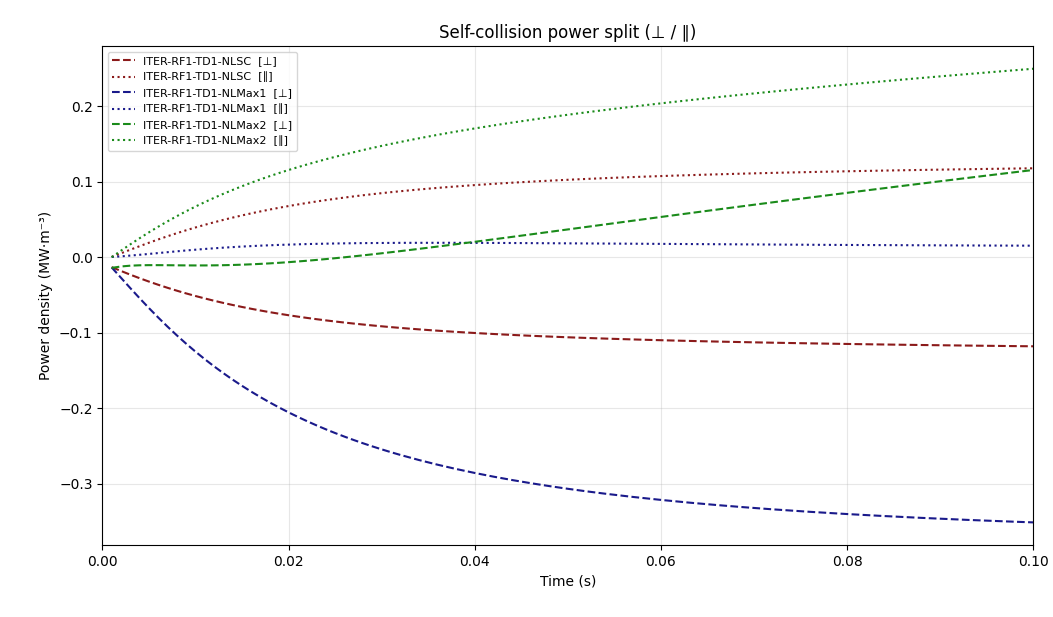
\includegraphics[width=0.75\textwidth]{../sc_power_split-comps.png}
  \caption{Self-collision power split $P_{\mathrm{SC},\perp}$ (dashed) and
    $P_{\mathrm{SC},\parallel}$ (dotted) vs time. For \texttt{isc=2} (green) the
    perpendicular component flips from sink to source at $t\approx0.04$\,s.}
  \label{fig:scsplit}
\end{figure}

The sign flip is understood as follows. At $t=0$ the distribution is the
$12$\,keV Maxwellian, so $T_b\approx T_\text{eff}\approx$ the bulk temperature
and $f\approx f_M(T_b)$: the operator is nearly null. As RF heats $v_\perp$, $f$
first becomes anisotropic while $T_\text{eff}$ is still near the bulk, and the
operator does ordinary isotropisation ($\perp\!\to\!\parallel$): hence
$P_{\mathrm{SC},\perp}<0$ and $P_{\mathrm{SC},\parallel}>0$ initially, like the
exact operator. As $T_\text{eff}$ climbs above the bulk core, the spurious
heating of Test~2 switches on and grows, adding a positive contribution to
both channels; in $\perp$ it eventually overtakes the isotropisation sink and
$P_{\mathrm{SC},\perp}$ crosses zero.

The crossover time is set by the \emph{ion self-collision time}. For the
tritium minority at $12$--$13.5$\,keV, $n_T = 7.5\times10^{19}$\,m$^{-3}$,
$\ln\Lambda\approx21.5$ (NRL formulary),
$\tau_{ii}\approx 29$--$35$\,ms --- right on the observed $\sim$40\,ms. (The RF
time to raise $T_\text{eff}$ by the $\sim$1.5\,keV needed to flip is comparable,
$\sim$30\,ms, as it must be at the crossover.) This gives a clean two-timescale
picture: a \emph{fast} clock, $\tau_{ii}\approx 30$--$40$\,ms, on which
self-collisions respond and the \texttt{isc=2} operator's character flips from
sink to source; and a \emph{slow} one, $\sim$seconds, on which the net energy
balance drives the runaway to $79$\,keV (set by the much weaker electron drag
plus the feedback). The pathology therefore announces itself within one
self-collision time and then drives the slow runaway.

% ---------------------------------------------------------------------------
\section{Further diagnostics not yet carried out}
% ---------------------------------------------------------------------------

Tests~1, 2 and~5 above have been carried out (Section~\ref{sec:tests}). The
following would further strengthen the analysis:

\begin{itemize}
  \item \textbf{Two background temperatures side by side.} Output both
        $T_\text{eff}$ (energy-weighted) and a density-characteristic
        temperature $T_n$ (e.g.\ from the curvature of $\ln f$ near the core,
        or a low-order moment dominated by the bulk). The gap
        $T_\text{eff}/T_n$ quantifies exactly how far the \texttt{isc=2}
        background departs from the collisionally-relevant temperature, and
        would let one test an ``\texttt{isc=2} with $T_b = T_n$'' variant.

  \item \textbf{Parallel and cross coefficients.} Add $D_{\parallel\parallel}$,
        $F_\parallel$ and the off-diagonal $D_{\perp\parallel}$ (slices and 2D
        maps) to confirm the anisotropic structure and check that the
        perpendicular channel is indeed the dominant error.

  \item \textbf{The Rosenbluth potentials $\psi$, $\phi$} (or their key
        $v_\perp$ derivatives) for the exact field vs.\ the two Maxwellian
        backgrounds, to visualise the root cause one level below $D$ and $F$.
\end{itemize}

% ---------------------------------------------------------------------------
\section{Conclusions}
% ---------------------------------------------------------------------------

\begin{enumerate}
  \item \textbf{\texttt{isc=1} tracks the exact operator at steady state;
        \texttt{isc=2} does not.} With identical solver settings,
        \texttt{isc=1} gives $T_\text{eff} = 19.4$\,keV and
        $P_\text{RF} = 1.13$\,MW\,m$^{-3}$, close to the exact
        \texttt{isc=-1} values ($22.2$\,keV, $1.25$\,MW\,m$^{-3}$), whereas
        \texttt{isc=2} gives $79$\,keV and $3.41$\,MW\,m$^{-3}$.

  \item \textbf{The failure is the background \emph{temperature}, not the
        linearisation.} \texttt{isc=1} and \texttt{isc=2} use the same
        linearised operator on the same non-Maxwellian $f$; only $T_b$
        differs. Neither conserves energy exactly, but with $T_b$ at the bulk
        temperature the residual is a small stabilising sink, whereas with
        $T_b = T_\text{eff}$ it is a large destabilising source
        ($P_\text{SC} = +3.49$\,MW\,m$^{-3}$).

  \item \textbf{Mechanism (from the $D$/$F$ diagnostics).} The collisional
        field is density-weighted and dominated by the cold bulk, so a
        bulk-temperature background reproduces the true friction and diffusion
        (Fig.~\ref{fig:dpepe_fpe}). $T_\text{eff}$ is energy-weighted and
        inflated by the perpendicular RF tail; using it makes the background
        too hot, giving broad diffusion and $\sim$5$\times$ too-weak friction.
        The operator then pumps perpendicular energy instead of relaxing it,
        and the $T_b = T_\text{eff}$ slaving closes a runaway feedback loop.

  \item \textbf{The inflated $P_\text{RF}$ is secondary,} driven by the
        artificially hot, broad perpendicular distribution improving the
        2nd-harmonic resonant coupling.

  \item \textbf{Recommendation.} \texttt{isc=2} as currently defined
        ($T_b = T_\text{eff}$) should not be used for RF-driven or otherwise
        non-Maxwellian distributions. If a self-consistent self-collision
        model cheaper than the full nonlinear operator is needed,
        \texttt{isc=1} (fixed bulk-temperature background) is far more
        reliable here. A possible improvement to \texttt{isc=2} would be to
        define its background temperature from a density-weighted measure
        $T_n$ rather than the energy-weighted $T_\text{eff}$ (diagnostic~3
        above).
\end{enumerate}

\end{document}
